\documentclass{article}
\usepackage{graphicx}
\usepackage{amsmath}
\usepackage{hyperref}
\usepackage{float}
\usepackage{xcolor}

\begin{document}

\title{Solutions to hw7 homework on Convex Optimization https://web.stanford.edu/class/ee364a/homework.html}
\author{Andrei Keino}
\maketitle

% 8.16, 9.30 - p. 519, 9.31, 

\section*{8.16}

Maximum volume rectangle inside a polyhedron. Formulate the following problem as a
convex optimization problem. Find the rectangle 
$$
\mathcal{R} = \{x \in R^n \; | \; l \preceq x \preceq u \}
$$

of maximum volume, enclosed in a polyhedron 
$\mathcal{P} = \{x \; | \; Ax \preceq b\}.$ The variables 
are $l, u \in R^n.$ Your formulation should not involve an exponential number of constraints. \\

Solution. A straightforward, but very inefficient, way to express the constraint $\mathcal{R} \subseteq \mathcal{P}$
is to use the set of $m 2^n$ inequalities $A v_i \leq b,$ where $v_i$ are $(2^n)$ corners of $\mathcal{R}.$ (If the
corners of a box lie inside a polyhedron, then the box does.) Fortunately it is possible
to express the constraint in a far more efficient way. Define 
$$
a_{ij}^+ = max\{a_{ij}, 0\}, \quad 
a_{ij}^- = max\{-a_{ij}, 0\}
$$
Then we have $\mathcal{R} \subseteq \mathcal{P}$ if and 
only if 
$$
\sum_{i = 1}^n (a_{ij}^+ u_j - a_{ij}^- l_j) \leq b_i, \quad i = 1, \dots, m 
$$

The maximum volume rectangle is the solution of
\begin{align*}
	&\text{maximize } && 
	(\prod_{i = 1}^n (u_i - l_i))^{1/n}
	\\
	&\text{subject to } 
	&& \sum_{i = 1}^n (a_{ij}^+ u_j - a_{ij}^- l_j) \leq b_i, \quad i = 1, \dots, m
\end{align*}

with implicit constraint $l \preceq u.$ 
Or after taking logarithm

\begin{align*}
	&\text{maximize } && 
	\sum_{i = 1}^n log(u_i - l_i)
	\\
	&\text{subject to } 
	&& \sum_{i = 1}^n (a_{ij}^+ u_j - a_{ij}^- l_j) \leq b_i, \quad i = 1, \dots, m
\end{align*}

\section*{9.30}
Gradient and Newton methods. Consider the unconstrained problem: \\
\begin{align*}
	&\text{minimize } && 
	f(x) = - \sum_{i=1}^m log(1 - a_i^T x) - 
	- \sum_{i=1}^n log(1 - x_i^2) \\
\end{align*}
with variable $x \in R^n$ and 
$\mathbf{dom} f =\{ x\; | \; a_i^T x < 1, \; 
i = 1, \dots, m, \; |x_i| < 1, \; i = 1, \dots, n \}$

This is the problem of computing the analytic center of the set of linear inequalities
$$
a_i^T x \leq 1, \quad i = 1, \dots, m, \quad |x_i| < 1, \quad i = 1, \dots, n
$$

Note that we can choose $x^{(0)} = 0$ as our initial point. You can generate instances of this
problem by choosing ai from some distribution on $R^n.$ \\

(a) Use the gradient method to solve the problem, using reasonable choices for the backtracking
parameters, and a stopping criterion of the form 
$||\nabla f||_2 \leq \nu.$ Plot the
objective function and step length versus iteration number. (Once you have determined $p^*$ to high accuracy, you can also plot $f - p^*$ versus iteration. Experiment
with the backtracking parameters $\alpha$ and $\beta.$ to see their effect on the total number of
iterations required. Carry these experiments out for several instances of the problem,
of different sizes. \\


(b) Repeat using Newton’s method, with stopping criterion based on the Newton decrement $\lambda ^ 2.$ Look for quadratic convergence. You do not have to use an efficient method
to compute the Newton step, as in exercise 9.27; you can use a general purpose dense
solver, although it is better to use one that is based on a Cholesky factorization.\\

Hint. Use the chain rule to find expressions for $\nabla f(x)$ and $\nabla_2 f(x)$.\\

Solution.\\

(a) Gradient descent. The python code:

\begin{verbatim}
# -*- coding: utf-8 -*-

# https://docs.scipy.org/doc/scipy/reference/generated/scipy.optimize.check_grad.html

# Convex optimization. gradient method.

import numpy as np
import matplotlib.pyplot as plt
plt.close('all')

#  definition of some functions ->
def gradient_numerical(f, x0, delta = 1e-8):
"""
function calculates the numerical gradient for function f in 
the point x0
"""
N = len(x0)
grad_num = np.zeros([N, 1])
for i in range(N):
xi_plus = x0.copy()
xi_plus[i] += delta

xi_minus = x0.copy()
xi_minus[i] -= delta

grad_num[i] = (f(xi_plus) - f(xi_minus)) / (2 * delta)       
return grad_num


def check_grad(f, gradf, x0, delta = 1e-8, verbose = True):
grad = np.array(gradf(x0))
grad_num = gradient_numerical(f, x0, delta)
if (verbose):
print('check_grad: precise gradient = ', grad)
print('check_grad: approximate gradient = ', grad_num)
print('check_grad: gradient error = ', grad - grad_num)        

return np.sqrt(np.sum((grad - grad_num) ** 2))


def f(x, a):
#  calculation of the function value
if not np.all(a.T @ x < 1):
return np.nan
if not np.all(np.abs(x) <= 1):
return np.nan
ret1 = - np.sum(np.log(1 - a.T @ x))  
ret2 =  - np.sum(np.log(1 - np.square(x)))
return ret1 + ret2


def gradf(x, a):
#  calculation of the function gradient

if not np.all(a.T @ x < 1):
return np.nan
if not np.all(np.abs(x) <= 1):
return np.nan
print('x = ', x)

ret1 = a @ (1 / (1 - a.T @ x))
ret2 = 2 * x * (1 / (1 - x ** 2))
return ret1 + ret2

def L2norm(x):
return np.sqrt(np.sum(x ** 2))

def backtrack(x, grad, alpha, beta):
"""
Backtracking line search
https://stackoverflow.com/questions/52204231/implementing-backtracking-line-search-algorithm-for-unconstrained-optimization-p
"""    
t = 1
while True: 
fx = f(x - t * grad, a)
fxx = f(x, a) + alpha * t * np.dot(grad.T, grad)
if np.isnan(fx) or np.isnan(fxx):
#  print('backtrack: nan detected; multilying t: t = ', t)
t *= beta
elif fx > fxx:
t *= beta
#  print('backtrack: multilying t: t = ', t)
else: 
#  print('backtrack: t found, returning: t = ', t)
return t

#  <- definition of some functions

np.random.seed(1)

m, n = 3, 2

a = np.random.random([m, n]).T

#  check the gradient calculation        

x_check = np.random.random([n, 1])

grad_err = check_grad(lambda x: f(x, a), lambda x: gradf(x, a), x_check)

assert grad_err < 1e-6, 'gradient calculation incorrect'

#  parameters for gradient descent method

nu_min = 1e-8 #  tolerance

step = 0.3

x_start = np.zeros([n, 1])

x = x_start


iter_num = 0

max_iters = 1000

max_line_search_iters = 1000

alpha = 0.4

beta = 0.4

print('x_start = ', x_start)
print('x_start.shape = ', x_start.shape)


t = backtrack(x, gradf(x, a), alpha, beta)
print('t after backtrack = ', t)

# the gradient descent implementation
while True:

print('iteration number ', iter_num)
grad = gradf(x, a)
nu = L2norm(grad)
print('nu = %e' % nu)
if nu <= nu_min:
print('gradient descent: tolerance achieved, exiting...')
print('iteration number ', iter_num)
print('optimal value = %e' % f(x, a))
print('optimal x = ', x)
break
#  Backtracking line search

t = backtrack(x, grad, alpha, beta)
step = t

print('step =', step)

print('grad = ', grad)

x = x - step * grad

print('new x = ', x)    
iter_num += 1
if iter_num >= max_iters:
print('gradient descent: max_iters number exeeded')
break


def gradient_descent(alpha, beta):

obj_func_arr = []
step_arr = []
iter_num = 0
x = x_start

while True:

print('iteration number ', iter_num)
obj_func_arr.append(f(x, a))
grad = gradf(x, a)
nu = L2norm(grad)
print('nu = %e' % nu)
if nu <= nu_min:
print('gradient descent: tolerance achieved, exiting...')
print('iteration number ', iter_num)
print('optimal value = %e' % f(x, a))
opt_val = f(x, a)
return np.array(obj_func_arr) - opt_val, step_arr
print('optimal x = ', x)
break
#  Backtracking line search

t = backtrack(x, grad, alpha, beta)
step = t

print('step =', step)

print('grad = ', grad)

x = x - step * grad
step_arr.append(step)

print('new x = ', x)    
iter_num += 1
if iter_num >= max_iters:
print('gradient descent: max_iters number exeeded')
return None, None
break

# plot the graphs        
alpha_arr = [0.2, 0.4]

beta_arr = [0.2, 0.45]

plt.figure()

for alpha in  alpha_arr:
for beta in beta_arr:
print('alpha = ', alpha)
print('beta = ', beta)
obj_func, step =  gradient_descent(alpha, beta)
x_plt = range(len(obj_func))
plt.plot(x_plt, np.log10(obj_func), 
label='alpha = ' + str(alpha) + ' beta = ' + str(beta))

plt.title('logarithm of the objective function error vs iteration number')
plt.ylabel('logarithm of the objective function error')
plt.xlabel('iteration number')
plt.legend()
plt.show()

plt.savefig('9_30_a_obj_func.png', bbox_inches='tight')


plt.figure()

for alpha in  alpha_arr:
for beta in beta_arr:
print('alpha = ', alpha)
print('beta = ', beta)
obj_func, step =  gradient_descent(alpha, beta)
x_plt = range(len(step))
plt.plot(x_plt, step, 
label='alpha = ' + str(alpha) + ' beta = ' + str(beta))

plt.title('step vs iteration number')
plt.ylabel('step')
plt.xlabel('iteration number')
plt.legend()
plt.show()

plt.savefig('9_30_a_step.png', bbox_inches='tight')

\end{verbatim}	

\begin{figure}[H]
	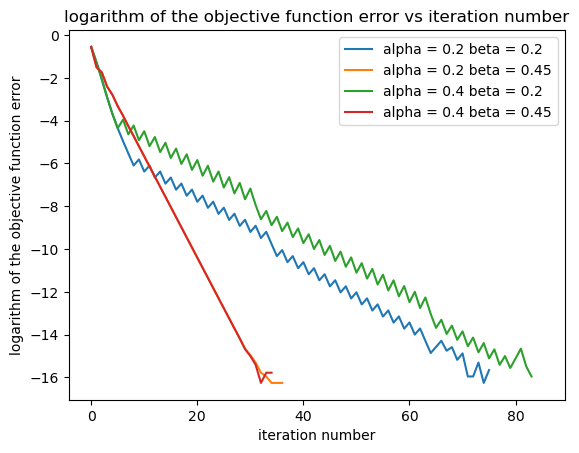
\includegraphics[width=\linewidth]{9_30_a_obj_func.png}
	\caption{Gradient descent: $f - p^*$ vs. iteration number}
\end{figure}

\begin{figure}[H]
	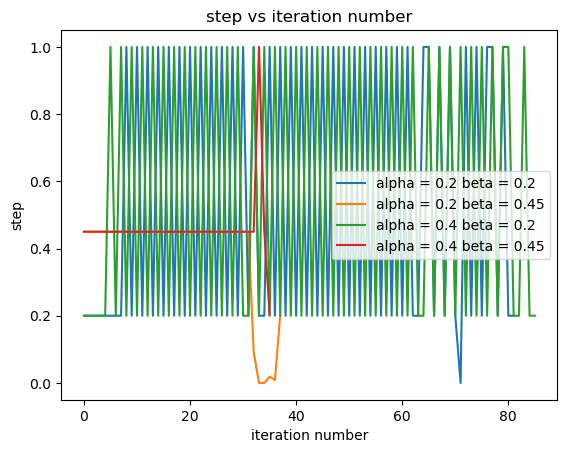
\includegraphics[width=\linewidth]{9_30_a_step.png}
	\caption{Gradient descent: step size vs. iteration number}
\end{figure}

(a) Newton's method. The python code: \\

file  \verb|ex_9_30_test_hessian.py|

\begin{verbatim}	
# -*- coding: utf-8 -*-
# https://docs.scipy.org/doc/scipy/reference/generated/scipy.optimize.check_grad.html

import numpy as np

def backtrack(x, a, grad, alpha, beta):
"""
Backtracking line search
https://stackoverflow.com/questions/52204231/implementing-backtracking-line-search-algorithm-for-unconstrained-optimization-p
"""    
t = 1
while True: 
fx = f(x - t * grad, a)
fxx = f(x, a) + alpha * t * np.dot(grad.T, grad)
if np.isnan(fx) or np.isnan(fxx):
#  print('backtrack: nan detected; multilying t: t = ', t)
t *= beta
elif fx > fxx:
t *= beta
#  print('backtrack: multilying t: t = ', t)
else: 
#  print('backtrack: t found, returning: t = ', t)
return t


def backtrack_2(x, a, grad, ihess, alpha, beta):
"""
Backtracking line search
https://stackoverflow.com/questions/52204231/implementing-backtracking-line-search-algorithm-for-unconstrained-optimization-p
"""
"""    
print('grad.shape = ', grad.shape)
print('grad = ', grad)
print('ihess.shape = ', ihess.shape)
print('ihess = ', ihess)
"""
gh = grad.T @ ihess
#  print('grad.T @ ihess = ', gh)


t = 1
while True: 
#  print('x = ', x)
#  print('gh = ', gh)

fx = f(x - t * gh , a)

fxx = f(x, a) + alpha * t * np.sum(gh ** 2)
#  fxx = f(x, a) + alpha * t * np.dot(gh, gh.T) #  the same as f(x, a) + alpha * t * np.sum(gh ** 2)

if np.isnan(fx) or np.isnan(fxx):
#  print('backtrack: nan detected; multilying t: t = ', t)
t *= beta
elif fx > fxx:
t *= beta
#  print('backtrack: multilying t: t = ', t)
else: 
#  print('backtrack: t found, returning: t = ', t)
return t

def L2norm(x):
return np.sqrt(np.sum(x ** 2))


def derivative_numerical(f, x0, i, delta = 1e-8):
xi_plus = x0.copy()
xi_plus[i] += delta

xi_minus = x0.copy()
xi_minus[i] -= delta
return (f(xi_plus) - f(xi_minus)) / (2 * delta)



def gradient_numerical(f, x0, delta = 1e-8):
"""
function calculates the numerical gradient for function f in 
the point x0
"""
N = len(x0)
grad_num = np.zeros([N, 1])
for i in range(N):
grad_num[i] = derivative_numerical(f, x0, i, delta)
return grad_num


def check_grad(f, gradf, x0, delta = 1e-8, verbose = True):
grad = np.array(gradf(x0))
grad_num = gradient_numerical(f, x0, delta)
if (verbose):
print('check_grad: precise gradient = ', grad)
print('check_grad: approximate gradient = ', grad_num)
print('check_grad: gradient error = ', grad - grad_num)        

return np.sqrt(np.sum((grad - grad_num) ** 2))

def second_derivative_numerical(f, x0, i, k, delta = 1e-5):
"""
function calculates second derivative
returns d^2f/(dx_k dx_i)
"""
xk_plus = x0.copy()
xk_plus[k] += delta

xk_minus = x0.copy()
xk_minus[k] -= delta

dfi_plus = derivative_numerical(f, xk_plus, i, delta)
dfi_minus = derivative_numerical(f, xk_minus, i, delta)

return (dfi_plus - dfi_minus) / (2 * delta)

def hessian_numerical(f, x0, delta = 1e-5):
"""
#  function calculates the hessian matrix
"""
assert x.shape[1] == 1, 'hessian_numerical: input array should have shape [N, 1]'

N = len(x)
hessian = np.zeros([N, N], dtype = np.float64)
for i in range(N):
for k in range(i, N):
hessian[i, k] = second_derivative_numerical(f, x0, i, k, delta)
if i != k:
hessian[k, i] = hessian[i, k]
return hessian

def check_hessian(f, hess_analytical, x0, delta = 1e-5, verbose = True):
"""
function checks he hessian matrix
"""
hessian_analytical = np.array(hess_analytical)
hessian_num = hessian_numerical(f, x0, delta)
if verbose:
print('check_hessian: hessian_analytical = ', hessian_analytical)
print('check_hessian: hessian_num = ', hessian_num)
print('check_hessian: hessian difference = ', 
hessian_analytical - hessian_num)

return np.sqrt(np.sum((hessian_analytical - hessian_num) ** 2))

#%%
# definitions for the function, gradient and hessian

def f(x, a):
#  calculation of the function value
if not np.all(a.T @ x < 1):
return np.nan
if not np.all(np.abs(x) <= 1):
return np.nan
ret1 = 0.0
ret1 = - np.sum(np.log(1 - a.T @ x))  
ret2 =  - np.sum(np.log(1 - np.square(x)))
return ret1 + ret2

#  print('f(x, a) = ', f(x, a))

def gradf(x, a):
#  calculation of the function gradient

if not np.all(a.T @ x < 1):
return np.nan
if not np.all(np.abs(x) <= 1):
return np.nan
#  print('x = ', x)

ret1 = 0.0    
ret1 = a @ (1 / (1 - a.T @ x))
ret2 = 2 * x * (1 / (1 - x ** 2))
return ret1 + ret2

def hessf(x, a):
if not np.all(a.T @ x < 1):
return np.nan
if not np.all(np.abs(x) <= 1):
return np.nan
ret1 = 0
ret1 = a @ (a.T * (1 / (1 - a.T @ x) ** 2))
ret2 = 2 * (1 + x ** 2) / ((1 - x ** 2) ** 2)
ret2 = np.diagflat(ret2)

return ret1 + ret2


if __name__ == "__main__":

np.random.seed(1)

m, n = 3, 2

a = np.random.random([m, n]).T

#  a = np.array([[-1, 0], [0.5, - 0.5], [0.5, 0]], dtype = np.float64).T

x0 = 0.5 * np.ones([n, 1]) 
x = np.array([-0.25, 0.75], dtype = np.float64).reshape(- 1, 1)



print('a.shape = ', a.shape)


#  x = np.array([0.5, 0.75])

#x = np.array([-0.75, 0.5], dtype = np.float64).reshape(- 1, 1)

error1 = check_grad(lambda x: f(x, a), lambda x: gradf(x, a), x0)

assert error1 < 1e-6, 'error1 too big'

print('gradient error1 = ', error1)


x0 = - 0.5 * np.ones([n, 1]) 
fl3 = lambda x: (x[0]**2 + 3*x[1]*x[0] + 12)

def f3(x):
return (x[0]**2 + 3*x[1]*x[0] + 12)[0]

dfx1 = lambda x: (2*x[0] + 3*x[1])
dfx2 = lambda x: (3*x[0])

def gradf3(x):
return np.array([dfx1(x), dfx2(x)]).reshape([-1, 1])


error3 = check_grad(f3, gradf3, x0)

print('gradient error3 = ', error3)

assert error3 < 1e-6, 'error3 too big'

error4 = check_grad(f3, gradf3, x0)

print('gradient error4 = ', error4)

assert error4 < 1e-6, 'error4 too big'

#%%
# test function for hessian 

def fh(z):
assert z.shape[0] == 2 and z.shape[1] == 1, 'fh(x): incorrect input shape'

x = z[0]
y = z[1]

return x**2 + 0.5 * y**2 + 2 * x * y + 3 * x + 4 * x**2 * y**2 + 5 * y * x**2

def fh_hessian(z):
assert z.shape[0] == 2 and z.shape[1] == 1, 'fh_hessian(x): incorrect input shape'

x = z[0]
y = z[1]

hessian = np.zeros([2, 2], dtype = np.float64)
print('')
hessian[0, 0] = 2 + 8 * y**2 + 10 * y
hessian[0, 1] = 2 + 16 * x * y + 10 * x
hessian[1, 0] = hessian[0, 1]
hessian[1, 1] = 1 + 8 * x ** 2
return hessian

#%%


#  test check_hessian function:

x0 = np.array([0.5, 8], dtype=np.float64).reshape(-1, 1)

#  x0 = np.array([0, 0], dtype=np.float64).reshape(-1, 1)

#  x0 = np.array([1, 1], dtype=np.float64).reshape(-1, 1)

hess_analytical = fh_hessian(x0)


hd = check_hessian(fh, hess_analytical, x0, delta = 1e-5, verbose = True)

print('test of check_hessian, diff = %e' % hd)

# x0 = np.array([0.5, -0.25], dtype=np.float64).reshape(-1, 1)    
x0 = np.array([-0.5, -0.75], dtype=np.float64).reshape(-1, 1)    

v_hess_analytical = hessf(x0, a)

print('v_hess_analytical = ', v_hess_analytical)


v_hess_num = hessian_numerical(lambda x: f(x, a), x0)

print('v_hess_num = ', v_hess_num)

hc = check_hessian(lambda x: f(x, a), v_hess_analytical, x0)
print('hc = ', hc)

assert hc < 1e-4, 'hessian seems to be incorrect'

grad = np.array([[3.26697727], [4.08950456]])    
ihess = np.array([[ 0.31264018, -0.13959122],  [-0.13959122,  0.28763308]])
print('grad.shape = ', grad.shape)
print('ihess.shape = ', ihess.shape)
y = grad.T @ ihess
print('y = ', y)
print('y.shape = ', y.shape)


print(np.sum(y**2))
\end{verbatim}	

file  \verb|ex_9_30_b.py|

\begin{verbatim}
# -*- coding: utf-8 -*-

import numpy as np
import ex_9_30_test_hessian as h
import matplotlib.pyplot as plt
plt.close('all')


f = h.f

np.random.seed(3)

m, n = 800, 60

a = np.random.random([m, n]).T


#  parameters for gradient descent method

nu_min = 1e-8 #  tolerance

step = 0.3

x_start = np.zeros([n, 1])

x = x_start


iter_num = 0

max_iters = 1000

max_line_search_iters = 1000

alpha = 0.4

beta = 0.4

print('x_start = ', x_start)
print('x_start.shape = ', x_start.shape)


# t = h.backtrack(x, a, h.gradf(x, a), alpha, beta)
# print('t after backtrack = ', t)

# the Newton's method implementation
while True:

print('iteration number ', iter_num)
grad = h.gradf(x, a) #  gradient of f
hess = h.hessf(x, a) #  hessian of f
ihess = np.linalg. inv(hess) #  inverse hessian of f
dx = - ihess @ grad #  Newton step
lam_sq = grad.T @ (ihess @ grad) # Newton decrement

print('lam_sq = %e' % lam_sq)
if np.sqrt(lam_sq / 2) <= nu_min:
print("Newton's method: tolerance achieved, exiting...")
print('iteration number ', iter_num)
#  print('a = ', a)
print('optimal value = %e' % f(x, a))
print('optimal x = ', x)
break
#  Backtracking line search

t = h.backtrack_2(x, a, grad, ihess, alpha, beta)
step = t
# step = 1

print('step =', step)

x = x + step * dx

print('new x = ', x)    
iter_num += 1
if iter_num >= max_iters:
print("Newton's method: max_iters number exeeded")
break


def newton_method(alpha, beta):

obj_func_arr = []
step_arr = []
iter_num = 0
x = x_start

while True:

print('iteration number ', iter_num)
obj_func_arr.append(f(x, a))
grad = h.gradf(x, a) #  gradient of f
hess = h.hessf(x, a) #  hessian of f
ihess = np.linalg. inv(hess) #  inverse hessian of f
dx = - ihess @ grad #  Newton step
lam_sq = grad.T @ (ihess @ grad) # Newton decrement

print('lam_sq = %e' % lam_sq)
#  if lam_sq / 2 <= nu_min:
if np.sqrt(lam_sq / 2) <= nu_min:
print("Newton's method: tolerance achieved, exiting...")
print('iteration number ', iter_num)
#  print('a = ', a)
opt_val = f(x, a)
print('optimal value = %e' % opt_val)
print('optimal x = ', x)
return np.array(obj_func_arr) - opt_val, step_arr            
break
#  Backtracking line search

t = h.backtrack_2(x, a, grad, ihess, alpha, beta)
step = t
step_arr.append(step)

print('step =', step)

x = x + step * dx

print('new x = ', x)    
iter_num += 1
if iter_num >= max_iters:
print("Newton's method: max_iters number exeeded")
return None, None
break

# plot the graphs        
alpha_arr = [0.2, 0.4]

beta_arr = [0.2, 0.45]

plt.figure()

for alpha in  alpha_arr:
for beta in beta_arr:
print('alpha = ', alpha)
print('beta = ', beta)
obj_func, step =  newton_method(alpha, beta)
x_plt = range(len(obj_func))
plt.plot(x_plt, np.log10(obj_func), 
label='alpha = ' + str(alpha) + ' beta = ' + str(beta))

plt.title('logarithm of the objective function error vs iteration number')
plt.ylabel('logarithm of the objective function error')
plt.xlabel('iteration number')
plt.legend()
plt.show()

plt.savefig('9_30_b_obj_func.png', bbox_inches='tight')


plt.figure()

for alpha in  alpha_arr:
for beta in beta_arr:
print('alpha = ', alpha)
print('beta = ', beta)
obj_func, step =  newton_method(alpha, beta)
x_plt = range(len(step))
plt.plot(x_plt, step, 
label='alpha = ' + str(alpha) + ' beta = ' + str(beta))

plt.title('step vs iteration number')
plt.ylabel('step')
plt.xlabel('iteration number')
plt.legend()
plt.show()

plt.savefig('9_30_b_step.png', bbox_inches='tight')
		
\end{verbatim}	

\begin{figure}[H]
	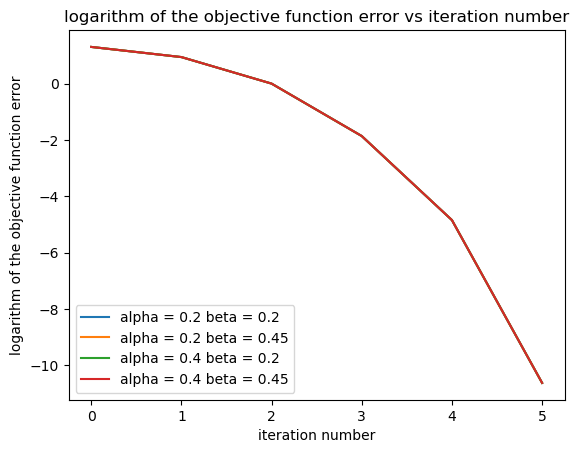
\includegraphics[width=\linewidth]{9_30_b_obj_func.png}
	\caption{Newton's method: $f - p^*$ vs. iteration number}
\end{figure}

\begin{figure}[H]
	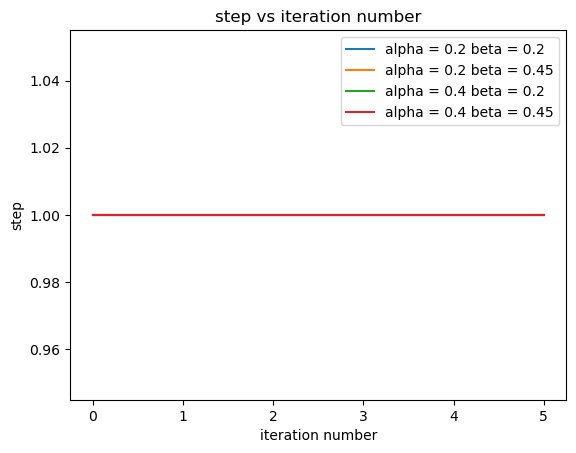
\includegraphics[width=\linewidth]{9_30_b_step.png}
	\caption{Newton's method: step size vs. iteration number}
\end{figure}


\section*{9.31}
Some approximate Newton methods. The cost of Newton’s method is dominated by the
cost of evaluating the Hessian $\nabla_2 f$ and the cost of solving the Newton system. For large
problems, it is sometimes useful to replace the Hessian by a positive definite approximation
that makes it easier to form and solve for the search step. In this problem we explore
some common examples of this idea.

For each of the approximate Newton methods described below, test the method on some
instances of the analytic centering problem described in exercise 9.30, and compare the
results to those obtained using the Newton method and gradient method.

(a) Re-using the Hessian. We evaluate and factor the Hessian only every $N$ iterations,
where $N > 1,$ and use the search step 
$\Delta x = - H^{-1} \nabla f(x),$ where $H$ is the last Hessian evaluated. (We need to evaluate and factor the Hessian once every $N$ steps; for the
other steps, we compute the search direction using back and forward substitution.)

(b) Diagonal approximation. We replace the Hessian by its diagonal, so we only have
to evaluate the n second derivatives 
$\frac{\partial^2 f(x)}{\partial t^2}$ and computing the search step is very easy.\\

Solution:

(a) The python code:

\begin{verbatim}
# -*- coding: utf-8 -*-

import numpy as np
import ex_9_30_test_hessian as h
import matplotlib.pyplot as plt
plt.close('all')


f = h.f

np.random.seed(3)

m, n = 18, 10

a = np.random.random([m, n]).T


#  parameters for gradient descent method

nu_min = 1e-8 #  tolerance

step = 0.3

x_start = np.zeros([n, 1])

x = x_start

max_iters = 1000

max_line_search_iters = 1000

alpha = 0.4

beta = 0.4

print('x_start = ', x_start)
print('x_start.shape = ', x_start.shape)

N = 3

iter_num = 0

# the Newton's method implementation

while True:

print('iteration number ', iter_num)

grad = h.gradf(x, a) #  gradient of f

"""
We need to evaluate and factor the Hessian once every N steps; for the
other steps, we compute the search direction using back and forward substitution
"""        
if iter_num // N == 0:
hess = h.hessf(x, a) #  hessian of f
ihess = np.linalg. inv(hess) #  inverse hessian of f

dx = - ihess @ grad #  Newton step
lam_sq = grad.T @ (ihess @ grad) # Newton decrement

print('lam_sq = %e' % lam_sq)
if np.sqrt(lam_sq / 2) <= nu_min:
print("Newton's method: tolerance achieved, exiting...")
print('iteration number ', iter_num)
#  print('a = ', a)
print('optimal value = %e' % f(x, a))
print('optimal x = ', x)
break
#  Backtracking line search

t = h.backtrack_2(x, a, grad, ihess, alpha, beta)
step = t
# step = 1

print('step =', step)

x = x + step * dx

print('new x = ', x)    
iter_num += 1
if iter_num >= max_iters:
print("Newton's method: max_iters number exeeded")
break

def newton_method(alpha, beta):

obj_func_arr = []
step_arr = []
iter_num = 0
x = x_start

while True:

print('iteration number ', iter_num)
obj_func_arr.append(f(x, a))

grad = h.gradf(x, a) #  gradient of f

"""
We need to evaluate and factor the Hessian once every N steps; for the
other steps, we compute the search direction using back and forward substitution
"""        
if iter_num // N == 0:
hess = h.hessf(x, a) #  hessian of f
ihess = np.linalg. inv(hess) #  inverse hessian of f

dx = - ihess @ grad #  Newton step
lam_sq = grad.T @ (ihess @ grad) # Newton decrement

print('lam_sq = %e' % lam_sq)
if np.sqrt(lam_sq / 2) <= nu_min:
print("Newton's method: tolerance achieved, exiting...")
print('iteration number ', iter_num)
#  print('a = ', a)
print('optimal value = %e' % f(x, a))
print('optimal x = ', x)
return np.array(obj_func_arr) - f(x, a), step_arr
break
#  Backtracking line search

t = h.backtrack_2(x, a, grad, ihess, alpha, beta)
step = t
step_arr.append(step)

print('step =', step)

x = x + step * dx

print('new x = ', x)    
iter_num += 1
if iter_num >= max_iters:
print("Newton's method: max_iters number exeeded")
break

# plot the graphs        
alpha_arr = [0.2, 0.4]

beta_arr = [0.2, 0.45]

plt.figure()

for alpha in  alpha_arr:
for beta in beta_arr:
print('alpha = ', alpha)
print('beta = ', beta)
obj_func, step =  newton_method(alpha, beta)
x_plt = range(len(obj_func))
plt.plot(x_plt, np.log10(obj_func), 
label='alpha = ' + str(alpha) + ' beta = ' + str(beta))

plt.title('logarithm of the objective function error vs iteration number')
plt.ylabel('logarithm of the objective function error')
plt.xlabel('iteration number')
plt.legend()
plt.show()

plt.savefig('9_31_a_obj_func.png', bbox_inches='tight')


plt.figure()

for alpha in  alpha_arr:
for beta in beta_arr:
print('alpha = ', alpha)
print('beta = ', beta)
obj_func, step =  newton_method(alpha, beta)
x_plt = range(len(step))
plt.plot(x_plt, step, 
label='alpha = ' + str(alpha) + ' beta = ' + str(beta))

plt.title('step vs iteration number')
plt.ylabel('step')
plt.xlabel('iteration number')
plt.legend()
plt.show()

plt.savefig('9_31_a_step.png', bbox_inches='tight')
	
\end{verbatim}	


\begin{figure}[H]
	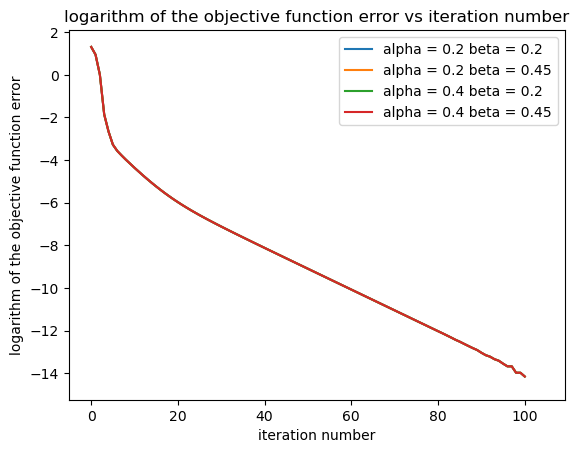
\includegraphics[width=\linewidth]{9_31_a_obj_func.png}
	\caption{Newton's method: $f - p^*$ vs. iteration number}
\end{figure}

\begin{figure}[H]
	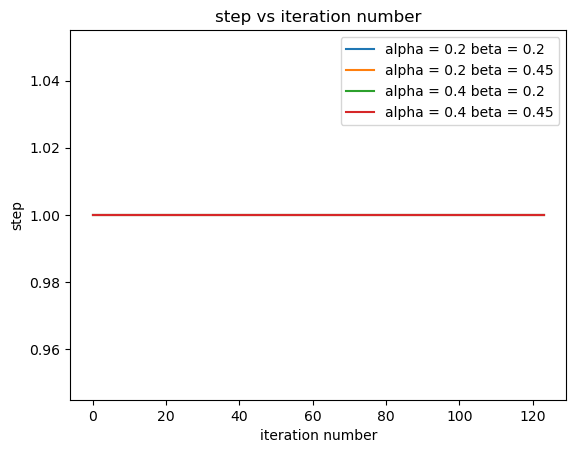
\includegraphics[width=\linewidth]{9_31_a_step.png}
	\caption{Newton's method: step size vs. iteration number}
\end{figure}

(b) The python code:

\begin{verbatim}
# -*- coding: utf-8 -*-

import numpy as np
import ex_9_30_test_hessian as h
import matplotlib.pyplot as plt
plt.close('all')

f = h.f

np.random.seed(3)

m, n = 18, 10

a = np.random.random([m, n]).T


#  parameters for gradient descent method

nu_min = 1e-8 #  tolerance

step = 0.3

x_start = np.zeros([n, 1])

x = x_start


iter_num = 0

max_iters = 1000

max_line_search_iters = 1000

alpha = 0.4

beta = 0.4

print('x_start = ', x_start)
print('x_start.shape = ', x_start.shape)


# the Newton's method implementation
while True:

print('iteration number ', iter_num)
grad = h.gradf(x, a) #  gradient of f
hess = h.hessf(x, a) #  hessian of f
# Diagonal approximation. We replace the Hessian by its diagonal
ihess = np.diag(1 / np.diagonal(hess))
# ihess = np.linalg. inv(hess) #  inverse hessian of f
dx = - ihess @ grad #  Newton step
lam_sq = grad.T @ (ihess @ grad) # Newton decrement

print('lam_sq = %e' % lam_sq)
if np.sqrt(lam_sq / 2) <= nu_min:
print("Newton's method: tolerance achieved, exiting...")
print('iteration number ', iter_num)
#  print('a = ', a)
print('optimal value = %e' % f(x, a))
print('optimal x = ', x)
break
#  Backtracking line search

t = h.backtrack_2(x, a, grad, ihess, alpha, beta)
step = t
# step = 1

print('step =', step)

x = x + step * dx

print('new x = ', x)    
iter_num += 1
if iter_num >= max_iters:
print("Newton's method: max_iters number exeeded")
break

def newton_method(alpha, beta):

obj_func_arr = []
step_arr = []
iter_num = 0
x = x_start


while True:

print('iteration number ', iter_num)
obj_func_arr.append(f(x, a))
grad = h.gradf(x, a) #  gradient of f
hess = h.hessf(x, a) #  hessian of f
# Diagonal approximation. We replace the Hessian by its diagonal
ihess = np.diag(1 / np.diagonal(hess))

dx = - ihess @ grad #  Newton step
lam_sq = grad.T @ (ihess @ grad) # Newton decrement

print('lam_sq = %e' % lam_sq)
if np.sqrt(lam_sq / 2) <= nu_min:
print("Newton's method: tolerance achieved, exiting...")
print('iteration number ', iter_num)
#  print('a = ', a)
print('optimal value = %e' % f(x, a))
print('optimal x = ', x)
return np.array(obj_func_arr) - f(x, a), step_arr
break
#  Backtracking line search

t = h.backtrack_2(x, a, grad, ihess, alpha, beta)
step = t
step_arr.append(step)

print('step =', step)

x = x + step * dx

print('new x = ', x)    
iter_num += 1
if iter_num >= max_iters:
print("Newton's method: max_iters number exeeded")
break

# plot the graphs        
alpha_arr = [0.2, 0.4]

beta_arr = [0.2, 0.45]

plt.figure()

for alpha in  alpha_arr:
for beta in beta_arr:
print('alpha = ', alpha)
print('beta = ', beta)
obj_func, step =  newton_method(alpha, beta)
x_plt = range(len(obj_func))
plt.plot(x_plt, np.log10(obj_func), 
label='alpha = ' + str(alpha) + ' beta = ' + str(beta))

plt.title('logarithm of the objective function error vs iteration number')
plt.ylabel('logarithm of the objective function error')
plt.xlabel('iteration number')
plt.legend()
plt.show()

plt.savefig('9_31_b_obj_func.png', bbox_inches='tight')


plt.figure()

for alpha in  alpha_arr:
for beta in beta_arr:
print('alpha = ', alpha)
print('beta = ', beta)
obj_func, step =  newton_method(alpha, beta)
x_plt = range(len(step))
plt.plot(x_plt, step, 
label='alpha = ' + str(alpha) + ' beta = ' + str(beta))

plt.title('step vs iteration number')
plt.ylabel('step')
plt.xlabel('iteration number')
plt.legend()
plt.show()

plt.savefig('9_31_b_step.png', bbox_inches='tight')		
\end{verbatim}	

\begin{figure}[H]
	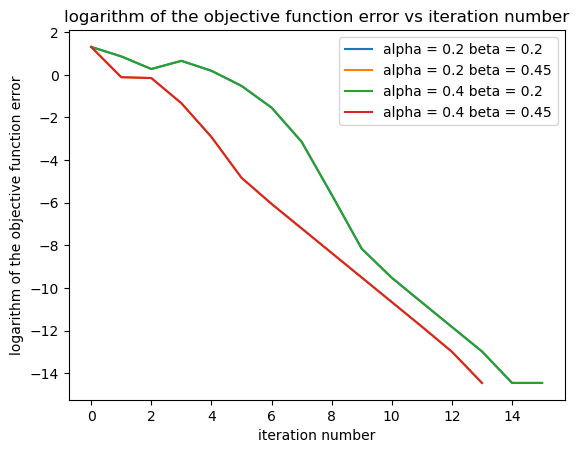
\includegraphics[width=\linewidth]{9_31_b_obj_func.png}
	\caption{Newton's method: $f - p^*$ vs. iteration number}
\end{figure}

\begin{figure}[H]
	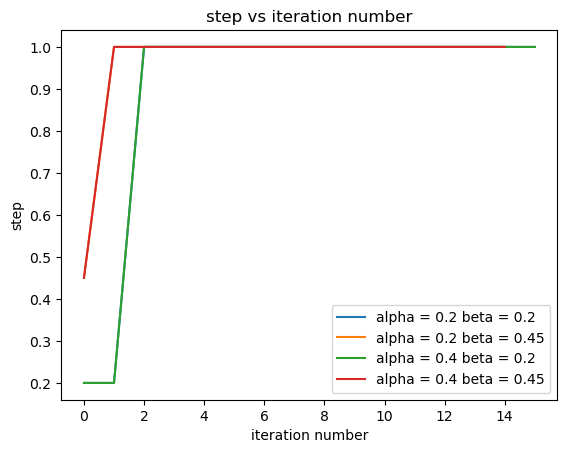
\includegraphics[width=\linewidth]{9_31_b_step.png}
	\caption{Newton's method: step size vs. iteration number}
\end{figure}


As it can be seen from the pictures, method (a) is not very good, but method (b) results somewhat 
comparable with the pure Newton's method ones.

\section*{Additional exercises}

\subsection*{1. Three-way linear classification.}

We are given data
$$
x^{(1)}, \dots, x^{(N)}, \quad
y^{(1)}, \dots, y^{(M)}, \quad
z^{(1)}, \dots, z^{(P)} \quad
$$

three nonempty sets of vectors in $R^n.$ We wish to find three affine functions on $R^n,$ 
$$
f_i(z) = a_i^T z - b_i, \quad i = 1, 2, 3,
$$

that satisfy the following properties:
\begin{align*}
	&f_1(x^{(j)}) > max\{f_2(x^{(j)}), f_3^{(x^{(j)})}\}, j = 1, \dots, N 
	\\
	&f_1(y^{(j)}) > max\{f_2(y^{(j)}), f_3^{(y^{(j)})}\}, j = 1, \dots, M 
	\\
	&f_1(z^{(j)}) > max\{f_2(z^{(j)}), f_3^{(z^{(j)})}\}, j = 1, \dots, P 
\end{align*}

In words: $f_1$ is the largest of the three functions on the x data points, $f_2$ is the largest of the three functions on the y data points, $f_3$ is the largest of the three functions on the $z$ data points. We can give a simple geometric interpretation: The functions $f_1$, $f_2$, and $f_3$ partition $R^n$ into three regions,

\begin{align*}
	R_1 = \{z\;|\; f_1(x) > max\{f_2(z), f_3(z)\}\} 
	\\
	R_2 = \{z\;|\; f_2(x) > max\{f_1(z), f_3(z)\}\} 
	\\
	R_3 = \{z\;|\; f_3(x) > max\{f_1(z), f_2(z)\}\} 
	\\
\end{align*}

defined by where each function is the largest of the three. Our goal is to find functions
with $x^{(j)} \in R^1,$ $y(j) \in R^2, $ and $z(j) \in R^3.$ Pose this as a convex optimization problem. You may not use strict inequalities in your formulation.

Solve the specific instance of the 3-way separation problem given in \verb|sep3way_data.m|,
with the columns of the matrices $X,$ $Y$ and $Z$ giving the $x^{(j)}, \; j = 1, \dots, N,$
$y^{(j)}, \; j = 1, \dots, M,$
$z^{(j)}, \; j = 1, \dots, P.$

To save you the trouble of plotting data points and separation boundaries, we have included the plotting code in \verb|sep3way_data.m|. (Note
that a1, a2, a3, b1 and b2 contain arbitrary numbers; you should compute the correct
values using cvx.)

{\bf Solution.} The inequalities

\begin{align*}
	&f_1(x^{(j)}) > max\{f_2(x^{(j)}), f_3^{(x^{(j)})}\}, j = 1, \dots, N 
	\\
	&f_1(y^{(j)}) > max\{f_2(y^{(j)}), f_3^{(y^{(j)})}\}, j = 1, \dots, M 
	\\
	&f_1(z^{(j)}) > max\{f_2(z^{(j)}), f_3^{(z^{(j)})}\}, j = 1, \dots, P 
\end{align*}
are homogeneous in $a_i$ and $b_i$ so we can express them as

\begin{align*}
	&f_1(x^{(j)}) > max\{f_2(x^{(j)}), f_3^{(x^{(j)})}\} + 1, j = 1, \dots, N 
	\\
	&f_1(y^{(j)}) > max\{f_2(y^{(j)}), f_3^{(y^{(j)})}\} + 1, j = 1, \dots, M 
	\\
	&f_1(z^{(j)}) > max\{f_2(z^{(j)}), f_3^{(z^{(j)})}\} + 1, j = 1, \dots, P 
\end{align*}

Note that we can add any vector to each of the $a_i$, without affecting these inequalities
(which only refer to difference between $a_i$’s), and we can add any number $\beta$ to each of
the $b_i$’s for the same reason. We can use this observation to normalize or simplify the
$a_i$ and $b_i$. For example, we can assume without loss of generality that $a_1 +a_2 +a_3 = 0$ and $b_1 + b_2 + b_3 = 0.$
The following script implements this method for 3-way classification and tests it on a
small separable data set

The following script implements this method for 3-way classification and tests it on a
small separable data set\\

\begin{verbatim}
clear all; close all;
% data for problem instance
M = 20;
N = 20;
P = 20;
X = [
3.5674 4.1253 2.8535 5.1892 4.3273 3.8133 3.4117 ...
3.8636 5.0668 3.9044 4.2944 4.7143 3.3082 5.2540 ...
2.5590 3.6001 4.8156 5.2902 5.1908 3.9802 ;...
-2.9981 0.5178 2.1436 -0.0677 0.3144 1.3064 3.9297 ...
0.2051 0.1067 -1.4982 -2.4051 2.9224 1.5444 -2.8687 ...
1.0281 1.2420 1.2814 1.2035 -2.1644 -0.2821];

Y = [
-4.5665 -3.6904 -3.2881 -1.6491 -5.4731 -3.6170 -1.1876 ...
-1.0539 -1.3915 -2.0312 -1.9999 -0.2480 -1.3149 -0.8305 ...
-1.9355 -1.0898 -2.6040 -4.3602 -1.8105 0.3096; ...
2.4117 4.2642 2.8460 0.5250 1.9053 2.9831 4.7079 ...
0.9702 0.3854 1.9228 1.4914 -0.9984 3.4330 2.9246 ...
3.0833 1.5910 1.5266 1.6256 2.5037 1.4384];

Z = [
1.7451 2.6345 0.5937 -2.8217 3.0304 1.0917 -1.7793 ...
1.2422 2.1873 -2.3008 -3.3258 2.7617 0.9166 0.0601 ...
-2.6520 -3.3205 4.1229 -3.4085 -3.1594 -0.7311; ...
-3.2010 -4.9921 -3.7621 -4.7420 -4.1315 -3.9120 -4.5596 ...
-4.9499 -3.4310 -4.2656 -6.2023 -4.5186 -3.7659 -5.0039 ...
-4.3744 -5.0559 -3.9443 -4.0412 -5.3493 -3.0465];

cvx_begin
variables a1(2) a2(2) a3(2) b1 b2 b3
minimize 0
subject to 
a1'*X-b1 >= max(a2'*X-b2,a3'*X-b3)+1;
a2'*Y-b2 >= max(a1'*Y-b1,a3'*Y-b3)+1;
a3'*Z-b3 >= max(a1'*Z-b1,a2'*Z-b2)+1;
a1 + a2 + a3 == 0
b1 + b2 + b3 == 0
cvx_end
a1
a2
a3
b1
b2
b3
% now let’s plot the three-way separation induced by
% a1,a2,a3,b1,b2,b3

% find maximally confusing point
p = [(a1-a2)';(a1-a3)']\[(b1-b2);(b1-b3)];
% plot
t = [-7:0.01:7];
u1 = a1-a2; u2 = a2-a3; u3 = a3-a1;
v1 = b1-b2; v2 = b2-b3; v3 = b3-b1;
line1 = (-t*u1(1)+v1)/u1(2); idx1 = find(u2'*[t;line1]-v2>0);
line2 = (-t*u2(1)+v2)/u2(2); idx2 = find(u3'*[t;line2]-v3>0);
line3 = (-t*u3(1)+v3)/u3(2); idx3 = find(u1'*[t;line3]-v1>0);
plot(X(1,:),X(2,:), '*',Y(1,:),Y(2,:),'ro',Z(1,:),Z(2,:),'g+',...
t(idx1),line1(idx1), 'k',t(idx2),line2(idx2),'k',t(idx3),line3(idx3),'k');
axis([-7 7 -7 7]);

% saveas(gcf,'additional_1_fig_1.png')

p = mfilename('fullpath')
[filepath,name,ext] = fileparts(p)
p
filepath

fname = strcat(filepath, '/additional_1_fig_1.png')
fname

saveas(gcf, fname)	
\end{verbatim}

\begin{figure}[H]
	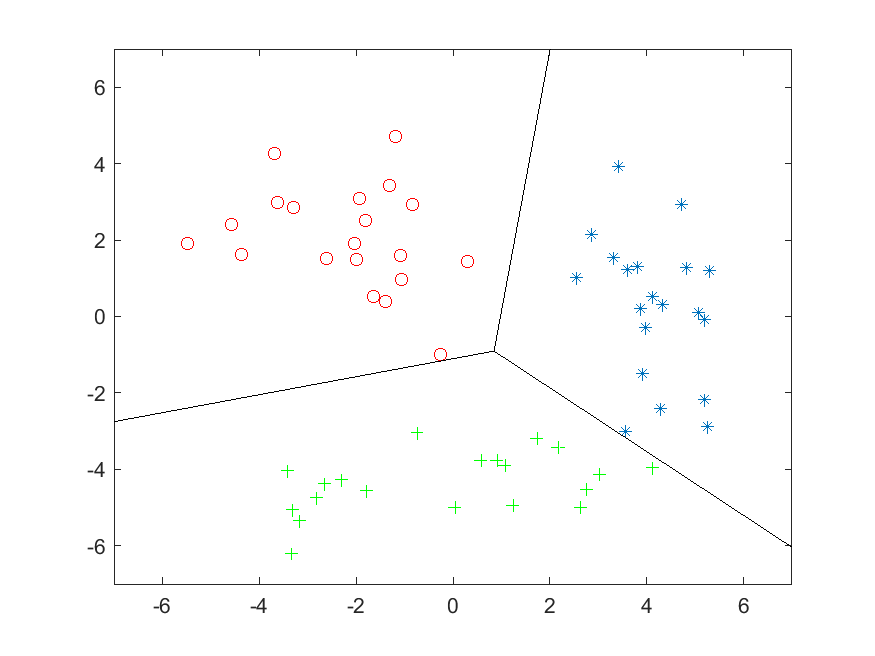
\includegraphics[width=\linewidth]
	{additional_1_fig_1.png}
	\caption{Three-way linear classification.}
\end{figure}


\subsection*{2. Efficient numerical method for a regularized least-squares problem.}

We consider a regularized least squares problem with smoothing,

$$
\text{minimize} \quad \sum_{i = 1}^{k} (a_i^T x - b_i)^2 
+ \delta \sum_{i=1}^{n-1}(x_i - x_{i-1})^2 + 
\eta \sum_{i=1}^n x_i^2
$$
where $x \in R^n$ is variable and $\eta, \delta > 0$ are parameters. \\

(a) Express the optimality conditions for this problem as a set of linear equations involving $x.$ (These are called the normal equations.)\\

(b) Now assume that $k \ll n.$ Describe an efficient method to solve the normal
equations found in (2a). Give an approximate flop count for a general method
that does not exploit structure, and also for your efficient method.\\

(c) A numerical instance. In this part you will try out your efficient method. We’ll
choose $k = 100$ and $n = 2000,$ and $\nu = \delta = 1.$ First, randomly generate $A$ and
$b$ with these dimensions. Form the normal equations as in (2a), and solve them
using a generic method. Next, write (short) code implementing your efficient
method, and run it on your problem instance. Verify that the solutions found by
the two methods are nearly the same, and also that your efficient method is much
faster than the generic one.\\

Note: You’ll need to know some things about Matlab to be sure you get the speedup
from the efficient method. Your method should involve solving linear equations with
tridiagonal coefficient matrix. In this case, both the factorization and the back sub-
stitution can be carried out very efficiently. The Matlab documentation says that
banded matrices are recognized and exploited, when solving equations, but we found
this wasn’t always the case. To be sure Matlab knows your matrix is tridiagonal, you
can declare the matrix as sparse, using \verb|spdiags|, which can be used to create a tridiagonal matrix. You could also create the tridiagonal matrix conventionally, and then convert the resulting matrix to a sparse one using \verb|sparse|.

One other thing you need to know. Suppose you need to solve a group of linear equations with the same coefficient matrix, \textit{i.e.}, you need to compute 
$F^{-1}a_1, \dots, F^{-1}a_m,$ where $F$ is invertible and $a_i$ are column vectors. concatenating columns, this can be expressed as a single matrix
$$
[F^{-1}a_1 \dots F^{-1} a_m] = F^{-1} [a_1 \dots a_m]
$$

To compute this matrix using Matlab, you should collect the righthand sides into one
matrix (as above) and use Matlab’s backslash operator: \verb|F\A|. This will do the right
thing: factor the matrix $F$ once, and carry out multiple back substitutions for the
righthand sides. \\

\textbf{Solution:}\\

(a)

The objective function is
$$
x^T ( A^TA + \delta \Delta + \eta I)x - 2b^T A x - b^Tb
$$
where $A \in R^{n \times k}$ is the matrix with rows $a_i,$ and $\Delta \in R{n \times n}$ is the tridiagonal matrix
$$
\Delta = \begin{bmatrix} 
	1 & -1 & 0  & \dots & 0 & 0 & 0 \\
	-1 & 2 & -1 & \dots & 0 & 0 & 0 \\
	0 & -1 & 2 & \dots & 0 & 0 & 0 \\	
	0 & 0  & 0 & \dots & 2 & -1 & 0 \\
	0 & 0 & 0 & \dots & -1 & 2 & -1 \\
	0 & 0 & 0 & \dots & 0  & -1 & 1 \\	
\end{bmatrix}
$$

Since the problem is unconstrained, the optimality conditions are

$$
(A^TA + \delta \Delta + \eta I)x^* - 2b^T A = 0
$$
or
$$
x^* = (A^TA + \delta \Delta + \eta I)^{-1} 2b^T A 
$$

(b)

If no structure is exploited, the nt cost of the solution is $1/3 n^3$ flops. If $k \ll n,$ we need to solve a system $Fx = g$ where $F$ is the sum of a tridiagonal
and a (relatively) low-rank matrix. We can use the Sherman-Morrison-Woodbury formula

$$
x^* = (\delta \Delta + \eta I)^{-1} g - 
(\delta \Delta + \eta I)^{-1} A^T 
(I + A(\delta \Delta + \eta I )^{-1} A^T)^{-1} A 
 (\delta \Delta + \eta I)^{-1} g
$$

to efficiently solve (1) as follows:

\begin{itemize}
	\item i. Solve $(\delta \Delta + \eta I) z_1 = g$ and 
	$(\delta \Delta + \eta I) Z_2 = A^T$ for $z_1$ and $Z_2.$ Since $(\delta \Delta + \eta I)$ is tridiagonal, the total cost is approximately 
	$4 nk + 5n$ flops ($n$ for factorization and $4n(k + 1)$ for the solves).	
	\item ii. Form $Az_1$ and $Az_2$ ($2 nk + nk^2$ flops).
	\item iii. Solve $(I + Az_2) z_3 = Az_1$ for $z_3$ 
	($1/3 k^3$ flops).
	\item iv. Form $x^* = z_1 - Z_2 z_3$ ($2nk$ flops).
	
\end{itemize}

The matlab code:
\begin{verbatim}
clear all; close all;
n = 2000;
k = 100;
delta = 1;
eta = 1;
A = rand(k,n);
b = rand(k,1);
e = ones(n,1);
D = spdiags([-e 2*e -e],[-1 0 1], n,n);

D(1,1) = 1; D(n,n) = 1;
I = speye(n);
F = A'*A + eta*I + delta*D;
P = eta*I + delta*D; %P is cheap to invert since it’s tridiagonal
g = A'*b;
%Directly computing optimal solution
fprintf('\nComputing solution directly\n');
s1 = cputime;
x_gen = F\g;
s2 = cputime;
fprintf('Done (in %g sec)\n',s2-s1);
fprintf('\nComputing solution using efficient method\n');
%x_eff = P^{-1}g - P^{-1}A’(I +AP^{-1}A’)^{-1}AP^{-1}g.
t1= cputime;
Z_0 = P\[g A'];
z_1 = Z_0(:,1);
%z_2 = A*z_1;
Z_2 = Z_0(:,2:k+1);
z_3 = (sparse(1:k,1:k,1) +A*Z_2)\(A*z_1);
x_eff = z_1 - Z_2*z_3;
t2 = cputime;
fprintf('Done (in %g sec)\n',t2-t1);
fprintf('\nrelative error = %e\n',norm(x_eff-x_gen)/norm(x_gen) );	
\end{verbatim}

\end{document}
